%% Copyright 2007, 2008, 2009 Elsevier Ltd

\documentclass[preprint,12pt]{elsarticle}

\usepackage{verbatim} % comentarios
\usepackage{epsfig}
\usepackage{amssymb} 

\usepackage{mathtools}

\usepackage{lineno}

\usepackage{tikz}        %permite rellenar las figuras (circulos)
\usepackage{etoolbox}
%\usepackage[backend=biber,citestyle=authoryear]{biblatex}
\usepackage{ulem}         %permite el tachado de texto.

%\usepackage{epstopdf}


\usepackage[caption=false]{subfig}

\begin{document}

\newcommand*{\hwplotB}{\raisebox{3pt}{\tikz{\draw[red,dashed,line 
width=3.2pt](0,0) -- 
(5mm,0);}}}

\newrobustcmd*{\mydiamond}[1]{\tikz{\filldraw[black,fill=#1] (0,0) -- 
(0.1cm,0.2cm) --
(0.2cm,0) -- (0.1cm,-0.2cm);}}

\newrobustcmd*{\mytriangleleft}[1]{\tikz{\filldraw[black,fill=#1] (0,0.15cm) -- 
(-0.3cm,0) -- (0,-0.15cm);}}
\definecolor{Blue}{cmyk}{1.,1.,0,0} 

\begin{frontmatter}


\title{Effects of the body force on the evacuation dynamics}


\author[add1]{I.M.~Sticco}
 \address[add1]{Departamento de F\'\i sica, Facultad de Ciencias 
Exactas y Naturales, \\ Universidad de Buenos Aires,\\
 Pabell\'on I, Ciudad Universitaria, 1428 Buenos Aires, Argentina.}

 \author[add2]{G.A.~Frank}
 \address[add2]{Unidad de Investigaci\'on y Desarrollo de las 
Ingenier\'\i as, Universidad Tecnol\'ogica Nacional, Facultad Regional Buenos 
Aires, Av. Medrano 951, 1179 Buenos Aires, Argentina.}

\author[add1,add3]{C.O.~Dorso\corref{cor1}}%
 \cortext[cor1]{codorso@df.uba.ar}

 \address[add3]{Instituto de F\'\i sica de Buenos Aires,\\
Pabell\'on I, Ciudad Universitaria, 1428 Buenos Aires, Argentina.}
 



\begin{abstract}

\end{abstract}

\begin{keyword}

Pedestrian Dynamics \sep Social Force Model \sep Body Force


\PACS 45.70.Vn \sep 89.65.Lm

\end{keyword}

\end{frontmatter}

%\linenumbers

\section{\label{introduction}Introduction}

\textcolor{red}{The Social Force Model (SFM) is a pedestrian dynamics model that
considers three kinds of forces: desired forces, social forces, and physical forces.
In its original version, the SFM, addresses two physical forces as essential: 
\sout{The Social Force Model (SFM) addresses two physical forces as 
\textit{essential}:}} the ``body force'' and the ``sliding friction''. Both are 
inspired by granular interactions and were claimed to be necessary  
for attaining the particular effects in panicking crowds \cite{helbing_2000}. 
The ``sliding friction'' actually proved to be an essential feature of the 
``faster-is-slower'' effect, although the role of the ``body force'' appears, 
at a first instance, not so clear \cite{dorso_2005,dorso_2007,dorso_2011}. \\ 

The existence of a ``body force'' in the context of highly dense crowds (say, 5 
to 10$\,$people/m$^2$) is a commonsense matter \cite{henein_2007,fruin_1993}. 
Researchers, however, question the numerical setting for this force in 
the SFM context \cite{lakoba_2005}. As a matter of fact, the usual setting by 
Helbing prevents the overlapping among pedestrians, but it is known to 
accomplish artificially high force levels 
\cite{helbing_2000,lakoba_2005,langston_2006,lin_2017}. The force estimates 
from the SFM appear to be remarkably higher with respect to the reported real 
life data (say, an order of magnitude). The crowd motion simulations, however, 
present quite realistic results \cite{lakoba_2005,langston_2006,dorso_2017}. 
The 
point seems to be that the SFM focuses on the \textcolor{red}{``collective behavior''
 \sout{``incoordination phenomenon''}} due 
to clogging, missing the ``individualistic'' perspective  of single pedestrians 
or very small groups \cite{helbing_2000,henein_2007,narain_2009}.  \\ 

Many researchers realized that modifying the SFM may (partially) surpass the 
misleading parameter setting. It was proposed that the pedestrians' 
psychological force (say, the ``social force'') should be suppressed in the 
context of highly dense crowds 
\cite{pelechano_2007,moussaid_2011,alonso_2014,bottinelli_2017}, or smoothly 
quenched according to the crowd density \cite{song_2019}. The authors in 
Refs.~\cite{kabalan_2017,jebrane_2019} further proposed a rigid body model in 
order to completely avoid the overlapping phenomenon. This perspective 
dismisses 
any connection to a ``sliding friction''. Conversely, other authors tried to 
limit the pedestrians acceleration by introducing ``static friction'' between 
the pedestrians and the floor \cite{wang_2019}. This kind of friction, however, 
reduces the effective willings of the pedestrians.  \\  

\textcolor{red}{A unique (and universal) setting appears not available yet. 
\sout{A meaningful (individualistic) numerical setting appears not available yet (to 
our knowledge).}} The reason is that different numerical settings can lead to 
the same crowd dynamics. Actually, only a small set of dimensionless 
``numbers'' control the crowd dynamics \cite{dorso_2019}. These are similar to 
those encountered in other active matter systems (P\'eclet number, etc.)  
\cite{marchetti_2014}. We may hypothesize that while the dimensionless 
``numbers'' provide some kind of control on the \textcolor{red}{\sout{
``incoordination phenomenon''} collective behavior} in 
crowds, only a few numerical settings can attain an ``individualistic'' 
meaning. 
 \\

The numerical setting for the ``faster is slower'' effect presented by 
Helbing and co-workers is somewhat cumbersome 
Ref.~\cite{helbing_2000,dorso_2017,dorso_2019}. Although a single 
parameter (say, the desired velocity $v_d$) is numerically varied to 
explain the phenomenon, the researcher looses sight of the dimensionless 
``numbers'' that truly control the crowd dynamics. The setting in 
Ref.~\cite{helbing_2000} also misses the ``faster is faster'' effect reported 
to occur at very high pedestrian densities \cite{dorso_2017,haghani_2019}. 
Alternatively, the empirical fundamental diagram raises as a point of reference 
for the SFM control parameters \cite{helbing_2007,dorso_2017}. \\

The fundamental diagram exhibits the flux behavior for either low dense crowds 
(with seldom contacts between pedestrians) and highly dense crowds (dominated 
by 
body forces and sliding friction). The latter usually experiences a flux 
slowing 
down, but other behaviors are also possible \cite{helbing_2007,lohner_2018}. In 
light of our previous hypothesis, we may suspect that the  modeling of the 
``flux slowing down'' within the context of the SFM will require the proper 
setting of the (dimensionless) controlling parameters. We examined this working 
hypothesis in Ref.~\cite{dorso_2019}, but limiting the parameter exploration to 
the sliding friction, disregarding the body force. \\

We now widen the investigation on the parameter settings to include the one 
associated to the body force. We will \textcolor{red}{\sout{focus} explore} 
on the complex interplay between 
the body force and the sliding friction among pedestrians. Recall that the 
interplay dynamics is not directly controlled by the numerical setting, but 
through dimensionless ``numbers'', where the model parameters appear mixed 
between each other. Thus, this step up offers a challenge to the 
``individualistic'' meaning of the parameter's setting. \\  


The investigation is organized as follows. We first recall the available 
experimental values on the body force and the sliding friction (see Section 
\ref{experimental}). Secondly, we introduce the reduced-in-units SFM and the 
three dimensionless numbers that control the crowd dynamics (see Section 
\ref{background}). We present our numerical simulations in Section 
\ref{results}. For the sake of clarity, this Section is 
separated into two major parts: the bottleneck scenario and the corridor 
scenario in Sections \ref{bottleneck} and \ref{corridor}, respectively. 
Section \ref{discussion} opens a detailed discussion raising from of the results 
in Section \ref{results}. The last Section closes the investigation with our 
main conclusions.

\section{\label{experimental}Experimental background}

The complex behavior of pedestrians \textcolor{red}{\sout{feature} features}
 either his (her) feelings and 
the environmental conditions. The former is expressed, for example, by his 
(her) moving ``attitude'' (say, self-assuredness). The latter brings out the 
observed separation between pedestrians. Also, the ``contacts'' between 
individuals address some kind of ``unwanted'' slowing down. All these 
observed patterns are commonly quantified in the literature into a set of 
characteristic  parameters. The experimental meaning of these parameters is as 
follows.

\begin{itemize}
\item[(i)] The walking attitude of a pedestrian may appear somewhat 
 \textcolor{red}{\sout{``assertive''} ``aggressive''} if he (she) reacts actively to unexpected behaviors 
\cite{lakoba_2005,helbing_1995}. The smaller the reaction time, the more 
\textcolor{red}{\sout{assertive or}}  aggressive observed posture. The associated parameter to this 
behavior is the relaxation or characteristic time $\tau$ 
\cite{johansson_2009,helbing_2000}. 

\item[(ii)] Despite the reactive attitude $\tau$, the pedestrian addresses a 
``free'' (undisturbed) walking speed $v_0$. This speed expresses his (her) 
motivation or intention to reach a certain destination (as comfortable as 
possible). Observations commonly associate $0.6\,$m/s, $1\,$m/s or $1.5\,$m/s 
to relaxed, normal or nervous walking speeds, respectively  
\cite{helbing_1995,helbing_2000,li_2015}. 

\item[(iii)] The walking speed of pedestrians appears to be lower in a 
crowded walkway with respect to their usually expected ``free'' walking speeds 
\cite{weidmann_1992,lakoba_2005}. Pedestrians tend to reduce their speed within 
crowded environments because they perceive not enough space for taking a 
step  \cite{johansson_2009}. This (perceived) step distance 
is therefore an influential parameter on the pedestrians behavior. 
It is known as the characteristic length $B$.

\item[(iv)] Physical interactions occur in very crowded environments. The 
``body force''  and ``sliding friction'' can be introduced straight forward. 
This will be done in Section \ref{background}. But it is worth noting that 
both are associated to the moving difficulties (say, slowing down and 
obstructions) observed in contacting pedestrians. 

\end{itemize}


Table~\ref{table_data} shows a few empirical figures for the most common 
parameters. More data is available throughout the literature (see, for example, 
Refs.~\cite{hoogendoorn_2007,seyfried_2007,johansson_2007,moussaid_2009,
luber_2010,seer_2014,li_2015} ). We intentionally omitted data that assumes a 
specific mathematical model. The exhibited values should also be considered as a 
general purpose approach, since no distinction has been made on age, gender or 
cultural habits. \\

\begin{table}
\begin{tabular}{c@{\hspace{6mm}}c@{\hspace{6mm}}c@{\hspace{6mm}}c@{\hspace{6mm}}
c@{\hspace{14mm}}l}
 \hline
 $\tau$[s]   & $m$[kg]     & $v_d$[m/s]  &  $B$[m]  & $k_n$[kg/s$^2$] &  Refs. \\
 \hline
0.61         & ---         & 1.24 & $0.36+1.06\,v$ &  ---                 &  
 \cite{seyfried_2007} \\
0.50$^*$     & 80$^*$      & 1.34 & 0.50           &  ---                 &  
\cite{weidmann_1992,lakoba_2005}\\
---          & $67.5$      & 1.39 &  ---           &  $96.1 + 12694.1\,x$ & 
\cite{song_2019}\\
---          & $67.0$      & 1.39 &  ---           &  $97.0 + 29378.9\,x$ & 
\cite{song_2019}\\


\hline
\end{tabular}
\caption{The experimental data for the pedestrian parameters, as explained in 
Section~\ref{experimental}. The magnitude $v$ means de pedestrian velocity 
(m/s). The magnitude $x$ means the compression length (m). The upper row for 
Ref.~\cite{song_2019} corresponds data acquired in winter and the lower row to 
datas acquiquired in summer. The asterisk ($^*$) corresponds to reasonable 
estimates from the authors. }
\label{table_data}
\end{table}

A first examination of the figures in Table~\ref{table_data} shows that the 
choise $\tau\simeq0.6\,$s seems to be a reasonable estimation for the 
relaxation time, although this may vary with respect to gender or culture 
\cite{siddharth_2018}. Additionally, we confirm that normal pedestrians attain 
desired velocities around $1.3\,$m/s. \\

The reports from Refs.~\cite{seyfried_2007,weidmann_1992} do not include any 
values for the compressibility $k_n$ since these experiments were carried out 
under low density conditions. \textcolor{red}{\sout{Notice that the} The} 
minimum (perceived) step distance 
is $0.36\,$m \textcolor{red}{according to Ref.}\cite{seyfried_2007}, but the
 pedestrians seem to require larger 
distances when they walk faster. The commonly accepted value $B\simeq 
0.5\,$m is somewhat valid for walking speeds under $0.5\,$m/s 
\cite{seyfried_2007}. Higher walking speeds (say, $1\,$m/s) will require 
a step distance of $1.3\,$m for the pedestrians to feel that there is enough 
space to move along.     \\ 

The reported data from Ref.~\cite{song_2019} correspond to the crowded 
environment of the Beijing subway. This environment was not suitable for 
providing information on the step distance $B$, but estimates for the 
desired speed and the body compresibility could be achieved. The reported 
magnitude $k_n$ assesses either the clothes and the body compressibility. The 
final value, though, is linearly related to the compression $x$. \\

We measured the maximum attainable forces at the subway in Buenos Aires, 
Argentina. Our preliminary results show that pedestrians feel ``uncomfortable'' 
whenever a body force ranging from $5$ to $20\,$N is applied for at least ten 
minutes. Short lasting forces (say, less than 4 minutes) may also be perceived 
as ``uncomfortable'' for values ranging from $10$ to $30\,$N. We also recorded body 
forces up to $60\,$N during very short ``hits''. The comparison with the 
fittings provided by Ref.~\cite{song_2019} shows that these magnitudes 
accomplish densities around 5 people/m$^2$.     \\    

The maximum (realistic) compressions may be computed from the relation 
$F=k(x)\,x$ and the compressibility $k_n(x)$ reported in Table~\ref{table_data}. 
An ``uncomfortable'' body force \textcolor{red}{\sout{of $30\,$N}} can address compressions in the 
range of $0.030-0.055\,$m. Also, a ``hitting'' force of $60\,$N can address 
compressions between $0.045$ and $0.065\,$m. Thus, according to 
Table~\ref{table_data}, we may expect experimental values for $k_n(x)$ up to 
$1000\,$kg/s$^2$ (for $F=30\,$N), or, up to $1400\,$kg/s$^2$ (for $F=60\,$N). \\

Besides, no realiable values for the sliding friction $\kappa$ appears to be 
available in the literature (to our knowledge). We may presume, however, that 
the sliding friction approaches a fraction of the body force. We will come back 
to this issue in Section~\ref{background}. \\


\section{\label{background}Theoretical background}

\subsection{\label{sfm}The Social Force Model}

The Social Force Model (SFM) provides the necessary framework for simulating 
the collective dynamics of self-driven particles (\textit{i.e.} pedestrians). 
The pedestrians are considered to follow an equation of motion involving 
either ``socio-psychological'' forces and physical forces (say, granular 
forces). The equation of motion for any pedestrian $i$ (of mass $m_i$) reads

\begin{equation}
 m_i\,\displaystyle\frac{d\mathbf{v}_i}{dt}=\mathbf{f}_d^{(i)}+
 \displaystyle\sum_{j=1}^N\mathbf{f}_s^{(ij)}+
 \displaystyle\sum_{j=1}^N\mathbf{f}_g^{(ij)}\label{eqn_motion}
\end{equation}

\noindent where the subscript $j$ corrresponds to any neighboring pedestrian or 
the walls. The three forces $\mathbf{f}_d$, $\mathbf{f}_s$ and $\mathbf{f}_g$ 
are different in nature. The desire force $\mathbf{f}_d$ represents the 
acceleration (or deceleration) of the pedestrian due to his (her) own willings. 
The social force $\mathbf{f}_s$, intead, describes the tendency of the 
pedestrians to stay away from each other. The granular force $\mathbf{f}_g$ 
stands for either the sliding friction and the compression between 
pedestrians. \\

Notice that these forces are supposed to influence the behavior of the 
pedestrians in a similar fashion as mentioned in Section~\ref{experimental}. 
Thus, the set of (empirical) parameters described in Section~\ref{experimental} 
is expected to be also present in the SFM. These will appear in connection to 
the forces, although their meaning may be somewhat different. \\   

The pedestrians' own willing is modeled by the desire force $\mathbf{f}_d$. 
This force stands for the acceleration (deceleration) required to reach a 
certain position at the desired walking speed $v_d$. This involves, however, a 
personal attitude that makes him (her) appear more or less ``assertive''. As 
mentioned in Section~\ref{experimental}, the reaction time $\tau$  attains for 
this attitude. Thus, the desire force is modeled as follows

\begin{equation}
\mathbf{f}_d^{(i)}=m\,\displaystyle\frac{v_d^{(i)}\,
\hat{\mathbf{e}}_d^{(i)}(t)-
 \mathbf{v}^{(i)}(t)}{\tau}
\end{equation}


\noindent where $\hat{\mathbf{e}}(t)$ represents the unit vector pointing to 
the target position. $\mathbf{v}(t)$ stands for the pedestrian velocity at time 
$t$. \\

The tendency of any individual to preserve his (her) ``private sphere'' is 
accomplished by the social force $\mathbf{f}_s$. This force is expected to 
prevent the pedestrians from getting too close to each other (or to the walls) 
in a crowded environment. If he (she) perceives that there is not enough space 
to move, he (she) will decelerate or even move back. The model for this kind of 
``socio-psychological'' behavior is as follows

\begin{equation}
 \mathbf{f}_s^{(i)}=A\,e^{(R_{ij}-r_{ij})/B}\,\hat{\mathbf{n}}_{ij}
 \label{eqn_social}
\end{equation}

\noindent where $r_{ij}$ means the distance between the center of mass of the 
pedestrians $i$ and $j$, and $R_{ij}=R_i+R_j$ is the sum of the pedestrians 
radius. The unit vector $\hat{\mathbf{n}}_{ij}$ points from pedestrian $j$ to 
pedestrian $i$, meaning a repulsive interaction.\\ 

The net distance $|R_{ij}-r_{ij}|$ scales to the parameter $B$ in the 
expression (\ref{eqn_social}). This parameter plays the role of a fall-off 
length within the model, and thus, it may be somewhat connected to the 
(perceived) step distance mentioned in Section~\ref{experimental}. The 
parameter $A$, however, does not provide any direct link to other parameters 
mentioned there. \\    

The granular force (say, the sliding friction plus the body force) attain to 
the moving difficulties encountered in very crowded environments. The 
expression for the granular force is has been borrowed from other granular 
matter fields, as follows

\begin{equation}
 \mathbf{f}_g^{(ij)}=\kappa\,g(R_{ij}-r_{ij})\,
(\Delta\mathbf{v}^{(ij)}\cdot\hat{\mathbf{t}}_{ij})\,\hat{\mathbf{t}}_{ij}+
k\,g(R_{ij}-r_{ij})\,
\,\hat{\mathbf{n}}_{ij}\label{eqn_friction}
\end{equation}

\noindent where $g(R_{ij}-r_{ij})$ equals $R_{ij}-r_{ij}$ if $R_{ij}>r_{ij}$ and 
vanished otherwise. $\Delta\mathbf{v}^{(ij)}\cdot\hat{\mathbf{t}}_{ij}$ 
represents the difference between the tangential velocities of the sliding 
bodies (or between the individual and the walls).    \\

The sliding friction occurs in the tangential direction while the body force 
occurs in the normal direction. Both are assumed to be linear with respect to 
the net distance between contacting pedestrians. The sliding friction is also 
linearly related to the difference between the (tangential) velocities. The 
coefficients $\kappa$ (for the sliding friction) and $k_n$ (for the 
body force) are supposed to be related to the areas of contact and the clothes 
material, among others. \\

We stress that the expression (\ref{eqn_friction}) assumes fixed values for 
$\kappa$ and $k_n$. This may not be completely true according to 
Table~\ref{table_data}. The local density (and thus, the pedestrians' 
compression) may affect the compressibility parameter $k_n$ by more than an order 
of magnitude. We will vary $k_n$ (and $\kappa$) in order to explore this 
phenomenon. \\  


\subsection{\label{parameters}The parameters setting}

The numerical setting of the parameters may affect the dynamics of the 
pedestrians. Some settings, however, yield similar collective dynamics.
\textcolor{red}{\sout{In order to investigate these similarities, we} We}
 introduce unit-less magnitudes 
and proceed straightforward as indicated in \ref{appendix1}. We realize from 
\ref{appendix1} that only three (unit-less) parameters  are the true 
``control'' parameters for the collective dynamics. These are $\mathcal{A}$, 
$\mathcal{K}$, $\mathcal{K}_c$ as defined in \ref{appendix1}. Recall that 
$\mathcal{A}$ and $\mathcal{K}$ are precisely the same as in 
Ref.~\cite{dorso_2019}, but a novel $\mathcal{K}_c$ parameter has been 
introduced due to the body force.   \\

The logical relations between the unit-less parameters and the ``individual'' 
parameters can be studied by means of the Venn diagrams exhibited in 
Fig.~\ref{venn_diagram}. The parameters $\mathcal{A}$, $\mathcal{K}$ and 
$\mathcal{K}_c$ are represented as intersecting sets, and the ``individual'' 
parameters are represented as elements within each set. The shared elements 
between $\mathcal{A}$, $\mathcal{K}$ and $\mathcal{K}_c$ are placed inside de 
intersecting regions. \\


\begin{figure}[!htbp]
\centering
 
\subfloat[\label{venn_2parameters}]
{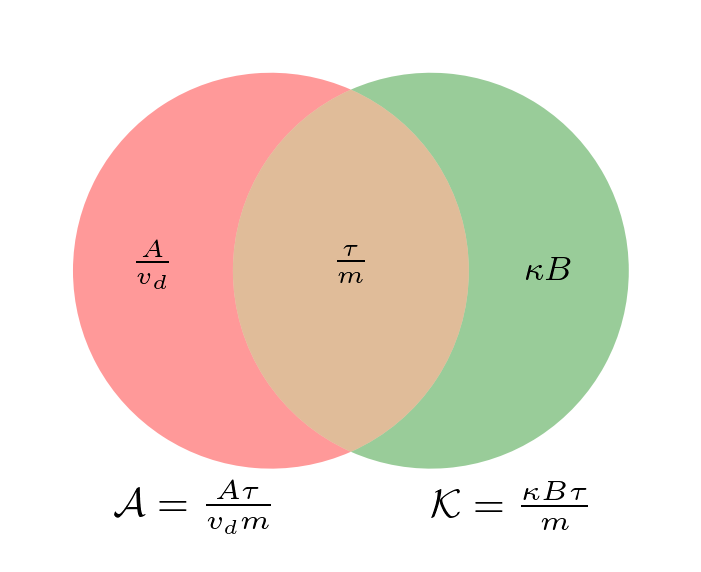
\includegraphics[width=0.45\columnwidth]{./venn_2parameters.png}}
\hfill    
\subfloat[\label{venn_3parameters}]
{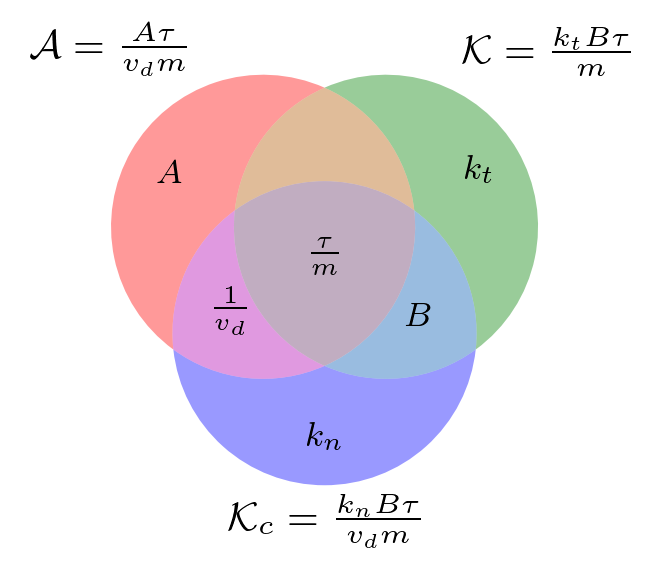
\includegraphics[width=0.45\columnwidth]{./venn_3parameters.png}
}\\
\caption[width=0.47\columnwidth]{Venn diagrams for the unit-less parameters
appearing in the equation of motion (\ref{eqn_motion}) (see 
Appendix~\ref{appendix1} for details). The sets correspond to 
$\mathcal{A}=\{\tau/m,1/v_d,A\}$, $\mathcal{K}=\{\tau/m,B,\kappa\}$ and 
$\mathcal{K}_c=\{\tau/m,1/v_d,B,k\}$. (a) The Venn diagram representation if no 
body force is introduced in the SFM (only sets $\mathcal{A}$ and $\mathcal{K}$, 
as in Ref.~\cite{dorso_2019}). (b) The Venn diagram representation for the sets 
$\mathcal{A}$, $\mathcal{K}$ and $\mathcal{K}_c$. }
\label{venn_diagram}
\end{figure}

A first inspection of the diagrams in Fig.~\ref{venn_diagram} shows that the 
relaxation time (per unit mass) $\tau/m$ is always a common parameter to all 
sets, regardless of the body force. This means that the ``assertive'' attitude 
of the pedestrian, addressed by the reaction time (see 
Section~\ref{experimental}), applies to all stimuli and the own willings. The 
role of $\tau$ has already been discussed in 
Refs.~\cite{johansson_2009,dorso_2019}.    \\ 

Fig.~\ref{venn_2parameters} represents the situation when $\mathcal{K}_c$ is 
absent. Notice that $A/v_d$ or $\kappa B$ may control the collective 
dynamic, in spite of the ``assertive'' attitude. The individual character of 
$v_d$ or $B$ appears somehow ``loosely'' in the crowd dynamic. We mean by 
``loosely'' that any numerical setting of these parameters may be 
counterbalanced by the right setting of $A$ or $\kappa$, keeping the 
colletive dynamic (qualitatively) unchanged.  \\

Fig.~\ref{venn_3parameters} provides a picture of the parameters' relations 
after introducing $\mathcal{K}_c$. Surprisingly, $\mathcal{K}_c$ appears as a
wider set (say, a four elements set) than $\mathcal{A}$ or $\mathcal{K}$ (three 
elements' sets). It shares the parameter $v_d$ with $\mathcal{A}$ and the 
parameter $B$ with $\mathcal{K}$. The practical consequence to these (logical)
relations is that $v_d$ or $B$ affect simultaneously two ``control'' parameters 
of the collective dynamics. Conversely, either $v_d$ and $B$ may counterbalance 
$\mathcal{K}_c$ in order to keep the colletive dynamic (qualitatively) 
unchanged.  \\

We confirm from these diagrams that no univocal relations can be established 
between the individual parameters and the collective dynamics (in a crowded 
environment). The presence of the body force moves the dynamics to a more 
complex context. We will investigate this context in section~\ref{results}. \\


\section{\label{results}Results}


\subsection{\label{bottleneck} Bottleneck}


We present in this section the results corresponding to the bottleneck geometry. 
We show the consequences of modifying the body force coefficient $k_n$ in the 
evacuation dynamics. Recall that this coefficient is associated 
to the compression of the human body. \\

Fig.~\ref{vd_vs_te} shows the evacuation time as a function of the pedestrian's 
desired velocity for different values of $k_n$. The evacuation 
time is defined as the time until 80\% of the pedestrians have 
left the room. In this section we will focus on the evacuation time for 
$2\,$m/s$<v_d<10\,$m/s.\\


\begin{figure}[htbp!]
\centering
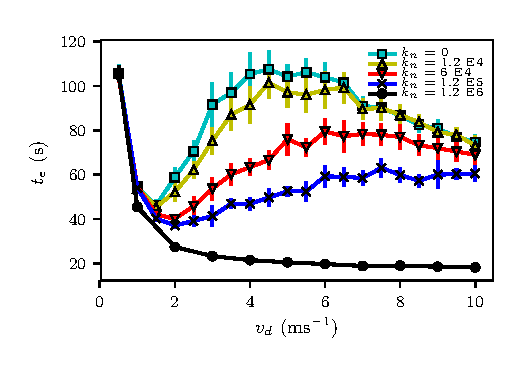
\includegraphics[width=0.7\columnwidth]
{./vd_vs_te_N225.eps}
\caption{\label{vd_vs_te}Mean evacuation time (s) vs. the pedestrian’s desired  
velocity (m/s) for a bottleneck. The room was 20 m x 20 m size. The door was 
0.92 m width. Mean values were computed from 10 evacuation processes. 225 
pedestrians were initially placed in a square lattice with a random initial 
velocity. Each process was finished when 158 pedestrians left the room. The 
different symbols indicate the $k_n$ value corresponding to the body force (see 
the label). The crosses correspond to the Helbing's original SFM parameter, the 
up-triangles correspond to the value measured in 
Ref.~\cite{anthropometric}, squares correspond 
to zero body force and circles correspond to an extreme value of stiffness (one 
order of magnitude higher than the original SFM). The 
 down triangles correspond to an intermediate value between the empirical value 
presented in Ref.~\cite{anthropometric} and the chosen by Helbing in 
Ref.~\cite{helbing_2000} }
\end{figure}

Two behavioral patterns can be seen in Fig.~\ref{vd_vs_te}. 
The region in which the slope is positive means that the 
harder the pedestrians try to get out (higher $v_d$), the 
longer it takes them to evacuate. This is the Faster-is-slower 
(FIS) regime. Conversely, the region in which the slope is 
negative  corresponds to a Faster-is-Faster (FIF) regime (the 
harder they try, the quicker they leave). Fig.~\ref{vd_vs_te} shows a change in 
in the behavior for desired velocities $v_d>1.2\,$m/s. The 
evacuation time is of type FIS+FIF for compression coefficients below 
$k=1.2\,$E5. This means that ``soft'' individuals are required to attain this 
behavioral change.  Notice that higher values of $k_n$ allow 
only FIS or FIF behaviors. For the highest explored value $k_n=1.2\,$E6, no 
FIS can be seen at all. Besides, the evacuation pattern for $k_n = 0$ and $k_n 
= 1.2\,$E4 are very similar since the body force is comparable to the social 
force for these stiffness values. \\

Despite the presence of the FIS or FIF phenomenon, the evacuation time at a 
fixed value of $v_d$ decreases for increasing values of $k_n$. This means that 
stiffer pedestrians evacuate faster than soft pedestrians. To investigate this 
issue, we computed the mean velocity of the whole crowd as a function of the 
stiffens $k_n$. Fig.~\ref{kn_vs_vx_bottleneck} shows the mean velocity in the 
x-direction as a function of the stiffness $k_n$ for three different desired 
velocities. In all cases, the velocity increases with the stiffness. From 
$k_n=0$ to $k_n=$1.2~E4 the increment of velocity is not as significative as it 
is for higher $k_n$. \\


\begin{figure}[!htbp]
\centering
    \subfloat[]{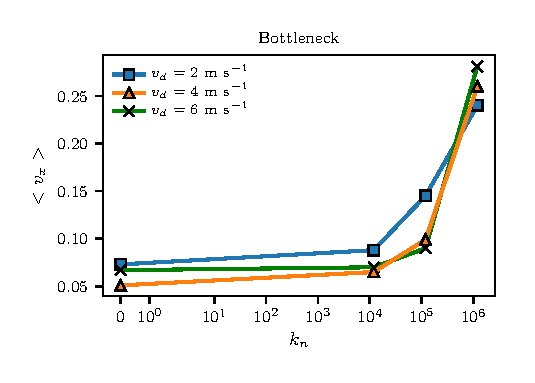
\includegraphics[width=0.7\columnwidth]{./kn_vs_vx_bottleneck.eps}}\\
\caption[width=0.47\columnwidth]{Mean velocity in the x-direction as a function 
of the stiffness level $k_n$ for different desired velocities (see label). The 
data corresponds to a bottleneck with periodic boundary conditions (re-injecting 
pedestrians). The average was taken every two seconds once the crowd reaches the 
stationary state ($t=$20~s) until the end of the simulation ($t=$110~s). }
\label{kn_vs_vx_bottleneck}
\end{figure}


The presence of a FIF phenomenon only for soft individuals opens many questions 
on the microscopic dynamics of pedestrians. We may presume that contacts 
between pedestrians are quite different for soft individuals than for stiff 
individuals. To study the dynamics of the contact, regardless of the compression 
effects, we assimilate the pedestrians as nodes and the whole crowd as a 
network. We set a link between any two individuals if both are in physical 
contact (\textit{i.e.} $r_{ij} \leq R{ij}$).\\

Fig.~\ref{degree_vd} shows the mean degree of the contact network as a function  
of the desired velocity. The degree of a node is defined as the number of links 
that connect this node to any other node. This means, the number of pedestrians 
that are in physical contact with a given pedestrian. The mean degree is the 
average of the degree over all the nodes (pedestrians) and over the whole 
sampled time. We report mean values after the system has reached the stationary 
state, that is after a well-formed bulk has been established.\\

Increasing $v_d$ increases the mean degree, as expected. This occurs because 
increasing $v_d$ produces higher densities that force individuals to touch each 
other. But surprisingly, for a given $v_d$, the mean degree reduces as the $k_n$ 
value increases. A noticeable decrease in the mean degree can be seen for the 
highest explored value of $k_n$. We may expect a significant change in the 
sliding friction due to this fact.\\

A more detailed insight into the contact dynamics can be acquired from 
Fig.~\ref{overlap_vd}. The overlap between individuals is shown as a function of 
$v_d$. Recall from section \ref{sfm} that the overlap is defined as 
$R_{ij}-r_{ij}$ where $R_{ij}$, is the sum of radius of particle $i$ and 
particle $j$ and $r_{ij}$  is the distance between both particles. Except for 
very low desired velocities (say, $v_d<2\,$m/s), we can see that the mean 
overlap is an increasing function of $v_d$ (for the studied $k_n$ values).\\

% Agregar valor de kappa en todos los captions. 

\begin{figure}[!htbp]
\centering
    \subfloat[]{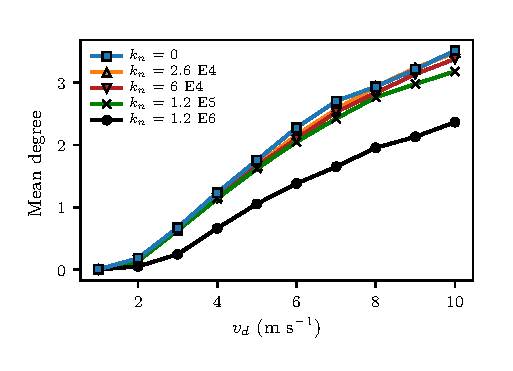
\includegraphics[width=0.45\columnwidth]{./degree_vs_vd_multi_kn.eps}\label{degree_vd}}\ 
    \subfloat[]{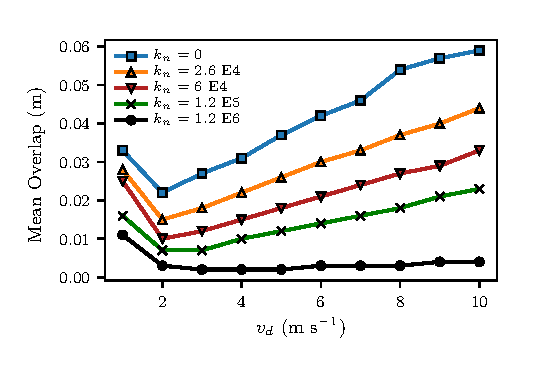
\includegraphics[width=0.45\columnwidth]{./overlap_vs_vd_multi_kn.eps}\label{overlap_vd}}\\
\caption[width=0.47\columnwidth]{(a) Mean degree as a function of the pedestrian’s desired velocity (m/s). (b) Mean overlap as a function of the pedestrians desired velocity. Each symbol indicates the $k_n$ value corresponding to the body force (see the labels). The data corresponds to a bottleneck with periodic boundary conditions (re-injecting pedestrians). The average was taken every two seconds once the crowd reaches the stationary state ($t=$20~s) until the end of the simulation ($t=$110~s).}
\label{degree_overlap_vd}
\end{figure}

The regime for $v_d<2\,$m/s is different from the rest since most of the 
pedestrians are not touching each other. The only pedestrians who touch each 
other are the ones who are being re-injected in the room. The overlap is higher 
than, for example, $v_d=3\,$m/s because of the pedestrians that 
are re-injected and collide with pedestrians in the bulk. \\

Besides, for a given $v_d$, the overlap increases as the $k_n$ value decreases. 
Reducing $k_n$ means reducing the normal body force, which allows a more 
significant intrusion of the personal space of the individuals 
(this means more overlap between pedestrians).\\  


Increasing the body stiffness has a significant impact on 
evacuation dynamics. The reduction of the overlap and the mean degree between 
pedestrians in the simulation, tend to diminish the sliding 
friction within the crowd. Consequently, an enhancement in the evacuation time 
(pedestrians escape faster) is observed, as pictured in Fig.~\ref{vd_vs_te}. 
Notice, however, that switching from a FIS regime (positive slope) to a  FIF 
regime (negative slope) in Fig.~\ref{vd_vs_te} appears as a more complex 
phenomenon. We will focus on this issue in an upcoming investigation.\\

Despite the effects on the sliding friction, the body force 
has a notorious impact in the number of pedestrians touching each other (say, 
the degree). This is clearly depicted in Fig.~\ref{network_bottleneck} where 
four different configurations of the evacuation dynamics are shown. The 
configurations represent 225 pedestrians trying to escape through a door see the 
caption for details. The colors correspond to the degree of each node 
(pedestrian), and the lines between pedestrians represent the contacts among 
them.\\



\begin{figure}[!htbp]
\centering
    \subfloat[]{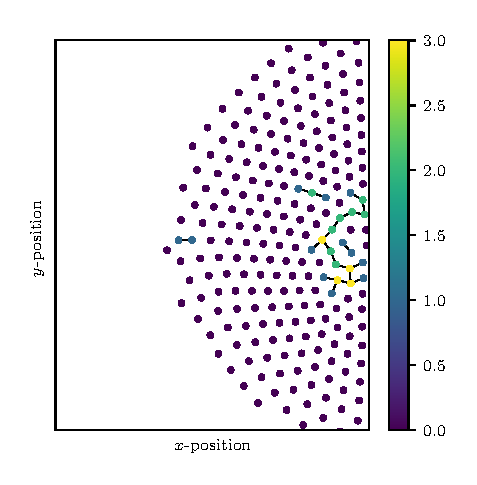
\includegraphics[width=0.45\columnwidth]{./network_vd2_kn0.eps}\label{network_vd2_kn0}}\ 
    \subfloat[]{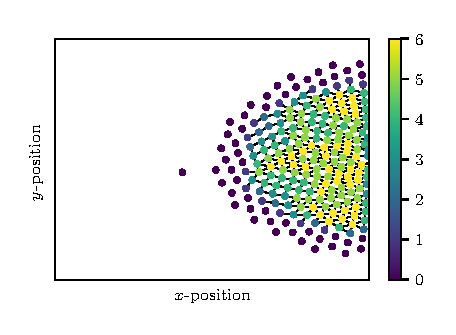
\includegraphics[width=0.45\columnwidth]{./network_vd10_kn0.eps}\label{network_vd10_kn0}}\\
        \subfloat[]{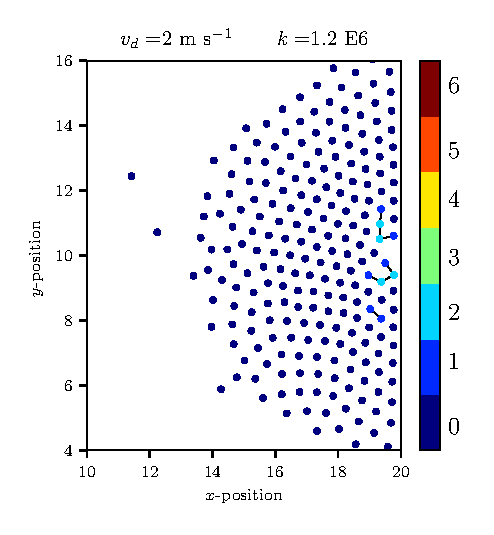
\includegraphics[width=0.45\columnwidth]{./network_vd2_kn1200000.eps}\label{network_vd2_kn1200000}}\ 
    \subfloat[]{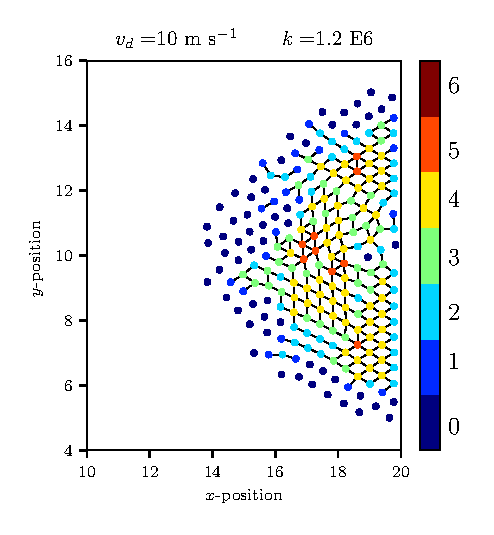
\includegraphics[width=0.45\columnwidth]{./network_vd10_kn1200000.eps}\label{network_vd10_kn1200000}}\\
\caption[width=0.47\columnwidth]{Contact networks of a 225 pedestrian evacuation through a bottleneck. The door is placed at $(x,y)=(20,10)$~m, the width of the door is 0.92~m (equivalent to 2 pedestrian\textsc{\char13}s diameter). The lines that connect the nodes (pedestrians) represent the contact between them. The color represents the degree (the number of pedestrians with which it is connected). (a) and (b) correspond to a simulation without body force with $v_d=$2 and $v_d=$10 respectively. (c) and (d) correspond to simulations with $k_n$=1.2~E6 with $v_d=$2 and $v_d=$10 respectively.}
\label{network_bottleneck}
\end{figure}



The four configurations corresponds to two different $v_d$ and two different $k_n$ values (say, the  minimum and maximum explored values). Fig.~\ref{network_vd2_kn0} and Fig.~\ref{network_vd10_kn0} shows a snapshot for $k_n=$0, at desired velocities of 2$\,$m/s and 10$\,$m/s respectively.    Fig.~\ref{network_vd2_kn1200000} and Fig.~\ref{network_vd10_kn1200000} show similar situations, but for  $k_n=$1.2$\,$E6. As expected, increasing the desired velocity compresses the crowd towards the exit. \\

The four snapshots in Fig.~\ref{network_bottleneck} confirm (visually) the fact that more rigid pedestrians release the crowded environment, widening the occupied region. At $v_d=10\,$m/s (the maximum explored velocity), it can hardly be found pedestrians with degree 6 when $k_n=1.2\,$E6, while a lot of them are present for $k_n$=0.\\

The clusterization of the pedestrians has a significant impact on the blocking clusters (the group of pedestrians that clog the exit).  Fig.~\ref{pbc_vs_vd_multi_kn} shows the blocking cluster existence probability as a function of the desired velocity for different $k$ values. The blocking clusters occur more often when the desired velocity increases because increasing $v_d$ increase the density in the area close to the exit. The most remarkable fact of Fig.~\ref{pbc_vs_vd_multi_kn} is that increasing the stiffness reduces the blocking cluster existence for a fixed value of $v_d$. Under these conditions, the blocking clusters strictly govern the evacuation dynamics~\cite{dorso_2005}. Thus, increasing the stiffness reduces the blocking cluster existence, which improves the evacuation time.\\

\begin{figure}[htbp!]
\centering
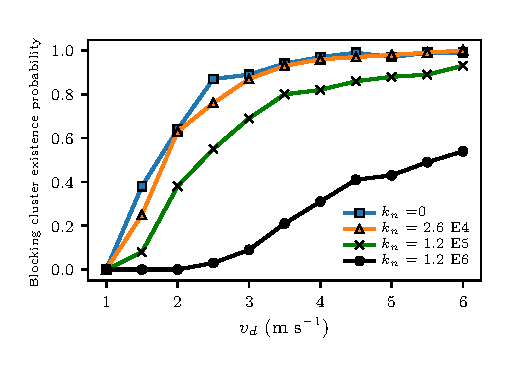
\includegraphics[width=0.7\columnwidth]
{./pbc_vs_vd_multi_kn.eps}
\caption{\label{pbc_vs_vd_multi_kn} Blocking cluster existence probability as a function of $v_d$ for different stiffness levels (see label). The probability is calculated as the amount of time a blocking cluster is present divided by the overall simulation time. The result correspond to a bottleneck geometry with 225 pedestrians in periodic boundary conditions (re-injection of pedestrians once the exited the room). The simulation lasted $t_f =$ 1000~s. }
\end{figure}


To conclude this section, we want to emphasize that increasing body stiffness has a significant impact on the evacuation dynamics. The stiffer pedestrians are, the less they touch to each other (less degree and less overlap). This phenomenon yields a reduction of the existence of the blocking clusters, which reduces the overall evacuation time. \\
\\

\subsection{\label{corridor} Corridor}

In this section, we present the results corresponding to the corridor geometry. We show the effects of modifying the body force coefficient $k_n$ in the dynamics.\\

In the same way as with the bottleneck geometry, we computed the contact network to study the topological differences that arise from increasing the $k_n$ value. Fig.~\ref{degree_dens} shows the mean degree as a function of the global density for different $k_n$ values. When the density is low,  the degree is zero because the pedestrians do not touch each other. When the density is around 4.5, a few pedestrians start to touch each other increasing the mean degree. As the density increases, the mean degree increases too until reaching an asymptotic behavior in degree six. Degree six, corresponds to the densest packing possible for identical hard circles, the result is a hexagonal packing arrangement.\\

It is important to notice that in Fig. \ref{degree_dens} for a given value of density, the stiffer the pedestrians, the higher the degree. In the bottleneck geometry, the opposite thing happens, the stiffer the pedestrians the lower the mean degree.\\

The mean overlap increases as the global density increases (see Fig. \ref{overlap_dens}) and the higher the stiffness the lower the overlap. This result is similar to the overlap vs. desired velocity obtained for bottleneck geometry. The higher the value of $k_n$ the higher the repulsion of the pedestrian-pedestrian interaction since the body force is acting in the normal direction $n_{ij}$.\\

\begin{figure}[!htbp]
\centering
    \subfloat[]{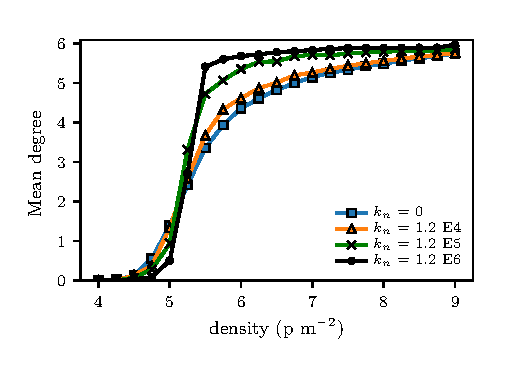
\includegraphics[width=0.45\columnwidth]{./degree_vs_dens_multi_kn.eps}\label{degree_dens}}\ 
    \subfloat[]{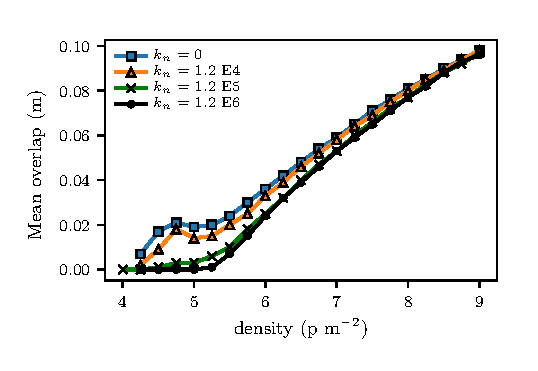
\includegraphics[width=0.45\columnwidth]{./overlap_vs_dens_multi_kn.eps}\label{overlap_dens}}\\
\caption[width=0.47\columnwidth]{(a) Mean degree as a function of the global density for different $k_n$ values. (b) mean overlap as a function of the global density. The mean values are averages over all the pedestrians and over time once the system reaches the stationary state. Both measurements correspond to corridor geometry with desired velocity $v_d=1$.}
\label{network_corridor}
\end{figure}

As was mentioned above, increasing the $k_n$ value of the body force increases the stiffness of pedestrians. Increasing the stiffness reduces the overlap (both in the bottleneck and corridor). Regarding the network connectivity, increasing the stiffness reduces the mean degree in a bottleneck but increases the mean degree in a corridor. Fig.~\ref{network_corridor} it shows the contact network corresponding to the corridor at a particular timestep and a particular global density. Fig.~\ref{network_d6_kn0} corresponds to $k_n=0$ while Fig.~\ref{network_d6_knE5} corresponds to $k_n=1.2$~E5. This is an example to show that increasing the stiffness increases the number of contacts between pedestrians (the network connectivity). Notice that there are many more pedestrians with degree 6 in the case of $k_n=1.2$~E5 than the case of $k_n=0$. \\

This result is exactly the opposite of what we get in the bottleneck. This happens because, in the corridor, the lateral walls act like containers that force the pedestrian to increase their contacts. Whereas in the bottleneck there are no lateral walls. Thus, when increasing the stiffness they have more space to detach from each other, reducing the connectedness (hence reducing the mean degree). \\

\begin{figure}[!htbp]
\centering
    \subfloat[]{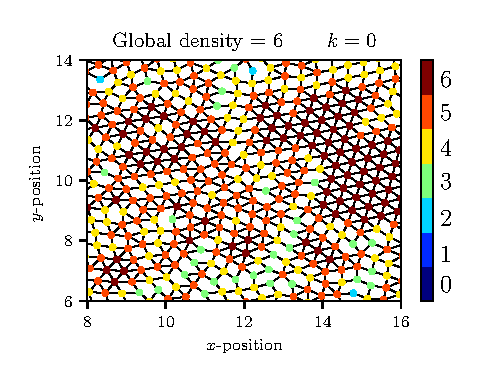
\includegraphics[width=0.45\columnwidth]{./network_d6_kn0.eps}\label{network_d6_kn0}}\ 
    \subfloat[]{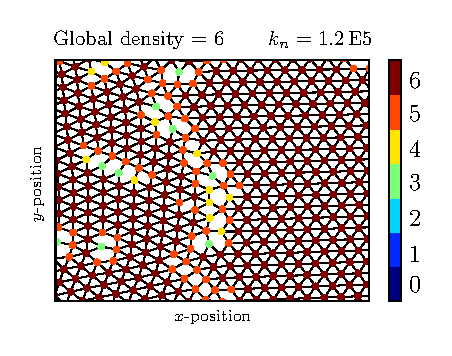
\includegraphics[width=0.45\columnwidth]{./network_d6_knE5.eps}\label{network_d6_knE5}}\\
\caption[width=0.47\columnwidth]{Contact network of the pedestrians along the corridor. The lines that connect the nodes (pedestrians) represent the contact between them. The colors stand for the degree of the node (the number of pedestrians that are in contact with him/her). The corridor was 28~m $\times$ 22~m with periodic boundary conditions and $v_d=1$. (a) corresponds to a simulation without body force and (b) corresponds to a simulation with $k_n=1.2$~E5.}
\label{network_corridor}
\end{figure}

In the corridor geometry, the crowd gets more connected if the pedestrians become stiffer. We studied the network properties of the contact graph arising from the positions $(x,y)$ of every pedestrian. We found that a good descriptor to exhibit the connectivity is the number of triangles per node. A triangle is defined as a structure composed of three nodes all in contact with each other. Fig.~\ref{triangles} shows the triangles per node as a function of the global density for different stiffness values $k_n$. This descriptor allows to distinguish states with the same global density but different stiffness levels. In other words, it is a descriptor very sensitive to changes in stiffness that allow expressing the connectivity of the system even better than the mean degree. \\

This result is consistent with the results obtained in Ref.~\cite{pugnaloni_2013} where the authors explore several topological and geometric descriptors capable of properly describing granular systems with different stiffness. While our study system is self-propelled, there are analogies with the system studied in Ref.~\cite{pugnaloni_2013} Like the authors, we recommend using topological descriptors (in particular triangles per node) to describe systems with equal global density and different stiffness levels.\\

\begin{figure}[htbp!]
\centering
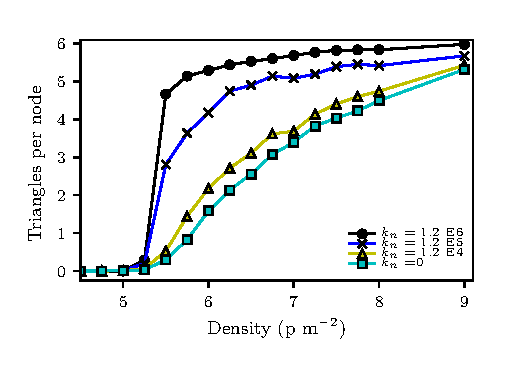
\includegraphics[width=0.7\columnwidth]
{./triangles.eps}
\caption{\label{triangles} Triangles per node as a function of the global density. A triangle in a network is defined as three nodes all connected. Each marker corresponds to a different stiffness $k_n$ (see the label in the plot). The measurements correspond to a corridor of 28~m $\times$ 22~m with periodic boundary conditions and $v_d=1$.  }
\end{figure}

The most important result is that increasing the $k_n$ value reduces the flow (hence reduces the walking speed of the overall crowd) in the corridor geometry. Fig.~\ref{kn_vs_vx_corridor} shows the velocity in the direction of displacement $v_x$ as a function of the stiffness for different global density levels. $v_x$ reduces as $k_n$ increases as opposed to what happens in the bottleneck geometry. There is little to no change in the speed from zero to $k_n=$1.2~E4, from this value on, the diminishing of velocity is more abrupt.\\

The reason why the velocity reduces as the stiffness of the pedestrians' increases is that it becomes harder for pedestrians to walk forward. The difficulty arises because the pedestrian feels a much higher repulsion from the pedestrian ahead (due to the body force increment). Thus, they have no other option than moving at (almost) the same speed as the pedestrians that they have at their sides. This microscopic mechanism explains the macroscopic behavior of the crowd that turns the crowd from a fluid-like state into a solid-like state. When the stiffness is high enough (say $k_n=$1.2~E6), all the pedestrians walk at the same velocity. The pedestrians that walk in physical contact with the wall are the ones who determine the velocity of the whole crowd.\\


\begin{figure}[htbp!]
\centering
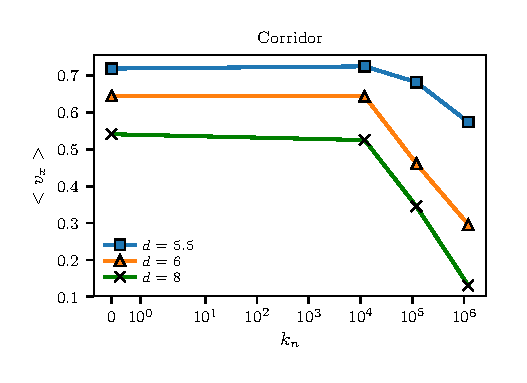
\includegraphics[width=0.7\columnwidth]{./kn_vs_vx_corridor.eps}
\caption{\label{kn_vs_vx_corridor} Mean velocity in the longitudinal coordinate $(v_x)$ as a function of the stiffness $k_n$ for three different global densities (see label in the plot). The measurements correspond to a corridor of 28~m $\times$ 22~m with periodic boundary conditions and $v_d=1$.      }
\end{figure}

The value of $k_n$ affects the velocity all along the corridor. Fig.~\ref{vx_profile} shows the velocity profile ($v_x$ vs. the longitudinal coordinate $y$) for different $k_n$ values. For $k_n=0$, we can see a parabolic-like velocity profile that resembles the Poiseuille flow (for Newtonian and incompressible fluids in laminar flow flowing through a pipe). As $k_n$ increases the velocity profile flattens until becoming a constant ($k_n=$ 1.2~E6) which $v_x$ value is much lower than on the case of soft pedestrians ($k_n=$0).\\

If the stiffness is high enough, the crowd behaves like a solid; this means that the crowd can not be easily deformed. In this context, to deform means to have parts of the crowd that move faster than other parts of the crowd. \\

The strain rate is a tensor for every point in the space. It expresses how the relative velocity of a medium changes when one moves away from a position in a specific direction. For this particular problem, we define the following version of the strain rate:

\begin{equation}
S = \frac{<v_x(center)> - <v_x(boundary)> }{\left | y(center) - y(boundary) \right |} 
\end{equation}

Where $<>$ means the average taken over time. By this definition we compare the velocity of the pedestrians close to the wall (boundary) with respect to the velocity of the pedestrians in the center of the corridor (center). As the stiffness level increases, the crowd becomes less deformable. This phenomenon is shown in Fig.~\ref{strain_rate_vs_kn} where we can see that the strain rate decreases with $k_n$. \\



\begin{figure}[!htbp]
\centering
    \subfloat[]{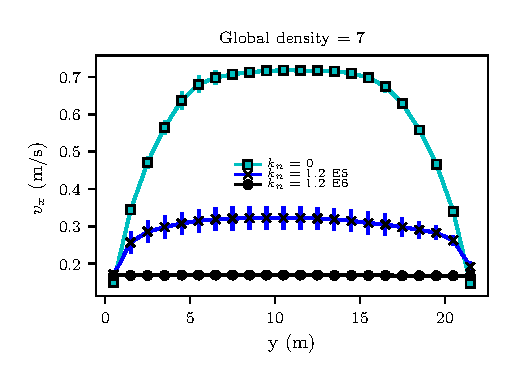
\includegraphics[width=0.45\columnwidth]{./vx_profile.eps}\label{vx_profile}}\ 
    \subfloat[]{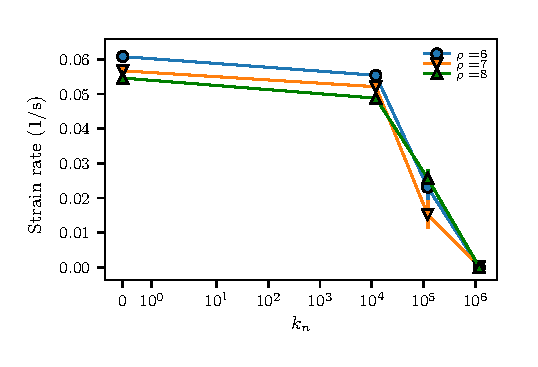
\includegraphics[width=0.45\columnwidth]{./strain_rate_vs_kn.eps}\label{strain_rate_vs_kn}}\\
\caption[width=0.47\columnwidth]{(a) Velocity in the $x$ coordinate as a function of the transversal coordinate $y$ for three different stiffness values $k$ (see the label). (b) Strain rate as a function of the stiffness level $k_n$ for three different global density values (see label). The measurements correspond to a corridor of 28~m $\times$ 22~m with periodic boundary conditions and $v_d=1$. The global density was 7 p~m$^{-2}$.  }
\label{profile_strain}
\end{figure}


\subsection{Dimensionless numbers and comparison with empirical data}


In this section, we inspect different values of the dimensionless numbers $\mathcal{K}_c$ and $\mathcal{K}$ and compare the results with the empirical measurements of Ref.~\cite{helbing_2007}. We varied the body force coefficient ($k_c$) and the friction coefficient ($k_t$) to inspect different values of $\mathcal{K}_c$ and $\mathcal{K}$ respectively.\\

The empirical measurements correspond to the fundamental diagram at the entrance of the Jamaraat bridge (see the inset in Fig.~\ref{flow_density_no_body_force}). We aim to reproduce the qualitative behavior of these measurements roughly.\\

Figs. \ref{flow_density} show the flow as a function of the global density (fundamental diagram). Fig.~\ref{flow_density_no_body_force} corresponds to $\mathcal{K}_c=$ 0 (zero body force \textit{i.e.} $k_n=0$) while Fig.~\ref{flow_density_body_force} corresponds to $\mathcal{K}_c=$68 (which is the value of the original SFM with $k_n$=1.2~E5 ). Each curve correspond to a different friction value, hence different $k_t$ value (see the caption).\\

According to most of the empirical measurements of the fundamental diagram, the flow decreases for high enough values of density because the crowd becomes jammed. Notice that the original friction (corresponding to $\mathcal{K}=$137) does not produce a reduction of the flow when there is zero body force ($\mathcal{K}_c$=0). Nevertheless, when the body force is included, and we remain the original friction (circles from Fig.~\ref{flow_density_body_force}), the flow reduces from  5 p m$^{-2}$ to 7 p m$^{-2}$ and then increases for higher values of density.\\

When the dimensionless number associated with the friction is $\mathcal{K} = $ 685 (the friction is five times the original SFM value), the flow reduces for densities higher than 5 p m$^{-2}$ in both cases (with body force and without body force). The main qualitative difference is that including the body force produces a subtle increment in the flow for densities higher than 7 p m$^{-2}$ (orange curve of Fig.~\ref{flow_density_no_body_force}). \\

When the dimensionless number associated to the friction is $\mathcal{K}=$1371  (the friction is ten times the original SFM value), in this case, the flow reduces or remains constant when the density is higher than 5 p m$^{-2}$ for both cases (with $\mathcal{K}_c=$ 0 and $\mathcal{K}_c = $ 68).\\

These results suggest that although increasing $\mathcal{K}_c$ produces a reduction in the flow, it is necessary to increase $\mathcal{K}$ (for instance, increasing friction $k_t$) to reproduce the reduction in the flow that characterizes the high-density regime. It is still a pending challenge to find the values of the dimensionless numbers that reproduce the qualitative behavior of the fundamental diagram, but this first approach narrows down the search.\\


\begin{comment}
Fig. \ref{flow_density} shows the flow as a function of the global density (fundamental diagram). \ref{flow_density_no_body_force} corresponds to zero body force (\textit{i.e.} $k_n=0$), Fig.~\ref{flow_density_body_force} corresponds to a body force with $k_n$=1.2~E5. Each curve correspond to a different friction value (see the caption).\\

According to most of the empirical measurements, the flow decreases for high enough values of density because the crowd becomes jammed. Notice that the original friction does not produce a reduction of the flow when there is zero body force but when the body force is included (with the original SFM value), the flow reduces from  5 p m$^{-2}$ to 7 p m$^{-2}$ and increases for higher values of density. When the friction is five times the original value, the flow reduces for densities higher than 5 p m$^{-2}$ in both cases (with body force and without body force). The main qualitative difference is that including the body force produces a subtle increment in the flow for densities higher than 7 p m$^{-2}$. When the friction is increased by a factor of ten, the flow reduces or remains constant when the density is higher than 5 p m$^{-2}$ for both cases (with body force and without body force). This result suggests that even including the body force, the original SFM requires an increment of the friction in order to reproduce the flow reduction reported in empirical measurements.\\
\end{comment}

\begin{figure}[!htbp]
\centering
    \subfloat[]{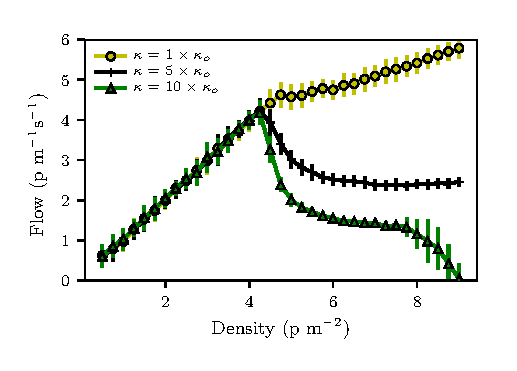
\includegraphics[width=0.45\columnwidth]{./flow-density_multifric_nobodyforce.eps}\label{flow_density_no_body_force}}\ 
    \subfloat[]{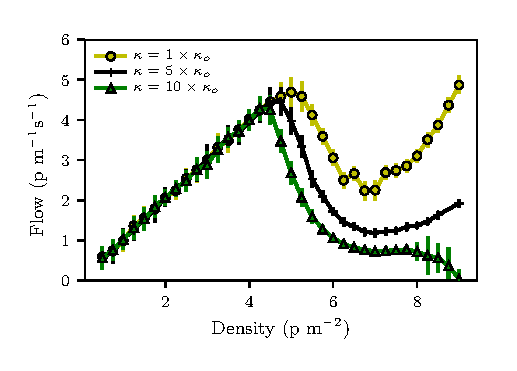
\includegraphics[width=0.45\columnwidth]{./flow-density_multifric_bodyforce.eps}\label{flow_density_body_force}}\\
\caption[width=0.47\columnwidth]{Flow vs. global density. The flow is calculated in a circular area of R=1~m at the center of the corridor. The circular markers correspond to the original friction of the SFM, the "+" symbol corresponds to the friction increased by a factor of five and the triangles correspond to the friction increased by a factor of ten. The desired velocity was $v_d=1$ in all the cases. (a) corresponds to simulations without body force ($\mathcal{K}_c =$0) and (b) corresponds to a body force with the original value of the body stiffness ($\mathcal{K}_c =$68).}
\label{flow_density}
\end{figure}


To conclude section \ref{results}, we remark that increasing the stiffness produces the opposite results in corridors respect to bottlenecks. The walls in the corridors play a critical role that prevents pedestrians from detaching from each other. This effect has consequences such as increasing the connectivity of the contact network, flattening the velocity profile (thus reducing the strain rate). If the stiffness is high enough, the pedestrians can not push to the pedestrian ahead since the body force repulsion becomes very high. This leads to a"solidification" of the crowd that makes all the pedestrians walk at almost the same velocity. The pedestrians that are in contact with the wall are the ones who determine the velocity of the whole crowd. \\


\section{\label{conclusions}Conclusions}


In this research, we explore the effect on the pedestrians dynamics of the (sometimes neglected) body force in the framework of the SFM. We showed that the stiffness coefficient ($k_n$) has a significant impact on the evacuation dynamics (bottleneck) and also in the dynamics of pedestrians walking along a straight corridor.\\

In the bottleneck geometry, the evacuation time diminishes (pedestrians move faster) as pedestrians become stiffer for all the ranges of the desired velocities explored. This phenomenon occurs because increasing the stiffness level promotes the repulsion between pedestrians pair interactions. As pedestrians detach from each other, the friction force diminishes due to the reduction of overlap between pedestrians and the contacts among them. The general decrease in frictional force reduces the probability of producing a cluster of pedestrians blocking the exist (blocking cluster), which leads to a more efficient evacuation dynamics. \\

In the corridor geometry, the actual walking speed reduces as pedestrians become stiffer. This is the opposite behavior with respect to the obtained in bottleneck geometry. The difference is explained because although increasing stiffness further separates individuals, they can not detach from each other as much as possible due to the lateral walls (these walls are not relevant in the bottleneck geometry). Thus, when the stiffness increases, the overlap between pedestrians is reduced while the number of contacts (degree) increases. Granular materials can behave like fluid or solids, depending on several conditions. If the stiffness level is low, the entire crowd behaves like a viscous fluid (with a parabolic velocity profile). However, if the stiffness level is high enough, the whole crowd behaves like a crystalline solid with a constant velocity profile which only depends on the friction interaction with the walls.\\

Regarding the parameters of the model, we found out that it is possible to reduce the original SFM parameters to three dimensionless parameters. The original parameters interrelate to each other through the dimensionless ones. Many different settings can produce the same dimensionless parameters. Thus, no univocal relations can be established between the individualistic parameters and collective dynamics.\\

\section*{Acknowledgments}
This work was supported by the National Scientific and Technical 
Research Council (spanish: Consejo Nacional de Investigaciones Cient\'\i ficas 
y T\'ecnicas - CONICET, Argentina) grant Programaci\'on Cient\'\i fica 2018 (UBACYT) Number 20020170100628BA.

\appendix

\section{\label{appendix1}Reduced-in-units equation of motion}

The SFM description in section~\ref{sfm} introduces seven parameters ($m$, 
$\tau$, $v_d$, $B$, $A$, $\kappa$ and $k_n$) attaining for the ``individual'' 
behavior of each pedestrian. The collective dynamic, however, requires a 
smaller set of parameters. In order to identify this smaller set, we introduce 
the following unit-less magnitudes\\

\begin{equation}
 \left\{\begin{array}{lcl}
         t' & = & t/\tau \\
         r' & = & r/B \\
         v' & = & v/v_d \\
        \end{array}\right.
\end{equation}

The equation of motion (\ref{eqn_motion}) can be written in terms of these 
(unit-less) magnitudes, while only three (reduced) parameters are needed.\\


\begin{equation}
 \displaystyle\frac{d\mathbf{v}'}{dt'}=
 \hat{\mathbf{e}}_d-\mathbf{v}'+\mathcal{A}\,e^{R'-r'}\,
 \hat{\mathbf{n}}+g(R'-r')\,\bigg[\mathcal{K}\,(\Delta\mathbf{v}'\cdot
 \hat{\mathbf{t}})\,\hat{\mathbf{t}}+\mathcal{K}_c\,\hat{\mathbf{n}}\bigg]
\end{equation}



\noindent where the smaller set ($\mathcal{A}$,$\mathcal{K}$,$\mathcal{K}_c$) 
means\\

\begin{equation}
 \mathcal{A}=\displaystyle\frac{A\,\tau}{m\,v_d}\ \ \ \ , \ \ \ \ 
 \mathcal{K}=\displaystyle\frac{\kappa\,B\,\tau}{m}\ \ \ \ , \ \ \ \
 \mathcal{K}_c=\displaystyle\frac{k\,B\,\tau}{m\,v_d}
\end{equation}

Notice that the SFM will arrive to similar collective dynamics whenever the 
reduced set ($\mathcal{A}$,$\mathcal{K}$,$\mathcal{K}_c$) remains unchanged 
(although some ``individual'' parameters are allowed to change). For a deep 
explanation on the meaning  of the set 
($\mathcal{A}$,$\mathcal{K}$,$\mathcal{K}_c$) see section~\ref{parameters}. \\




%/////////////////////////////////////////////////
%\begin{thebibliography}{10}
%\expandafter\ifx\csname url\endcsname\relax
%  \def\url#1{\texttt{#1}}\fi
%\expandafter\ifx\csname urlprefix\endcsname\relax\def\urlprefix{URL }\fi
%\expandafter\ifx\csname href\endcsname\relax
%  \def\href#1#2{#2} \def\path#1{#1}\fi

%\bibitem{helbing3}
%Helbing, D., Johansson, A., and Al-Abideen, H. Z., 2007. ``Dynamics of crowd 
%disasters: An empirical study." Physical review E 75 (4), 046109.
%{\path{https://doi.org/10.1103/PhysRevE.75.046109}}

%\end{thebibliography}

\bibliographystyle{unsrt}
\bibliography{paper}% Produces the bibliography via BibTeX.

\end{document}
\endinput

